
\documentclass[a4paper, 12pt]{article}
\usepackage{fullpage}
\usepackage[UTF8]{ctex}
\setCJKmainfont{Noto Serif CJK TC}

\usepackage{listings}
\usepackage{xcolor}

\lstdefinestyle{pythonstyle}{
    language=Python,
    basicstyle=\ttfamily\footnotesize,
    keywordstyle=\color{blue!70!black}\bfseries,
    commentstyle=\color{green!50!black}\itshape,
    stringstyle=\color{red!60!black},
    numberstyle=\tiny\color{gray},
    numbers=left,
    numbersep=6pt,
    frame=single,
    framesep=4pt,
    rulecolor=\color{gray!50},
    breaklines=true,
    showstringspaces=false,
    tabsize=4,
    columns=fullflexible,
    keepspaces=true,
    escapeinside={@}{@},   % 允許在程式碼中插入 LaTeX
}
\lstset{style=pythonstyle}

\usepackage{graphicx}
\usepackage{amsmath}
\usepackage{amsthm}
\usepackage{mathrsfs}
\usepackage{amssymb}
\usepackage{cancel}
\usepackage[ruled,vlined]{algorithm2e}

\usepackage{tikz}
\usepackage{subcaption}
\usetikzlibrary{positioning}
\usetikzlibrary{decorations.pathreplacing}
\usetikzlibrary{plotmarks,trees,arrows}
\usetikzlibrary{calc}
\usetikzlibrary{graphs}
\usetikzlibrary{shapes.geometric}
\usepackage{pgf}
\usepackage{color}

%% Theorem environments（定理環境）
\newtheorem{theorem}{Theorem}
\newtheorem{lemma}[theorem]{Lemma}
\newtheorem{corollary}[theorem]{Corollary}
\newtheorem{proposition}[theorem]{Proposition}
\newtheorem{definition}[theorem]{Definition}
\newtheorem{remark}[theorem]{Remark}
\newtheorem{claim}[theorem]{Claim}


%% TikZ styles（TikZ 樣式）
\tikzset{
    mynode/.style={draw,circle,fill=\c!30,scale=\s},
    root/.style={draw,rectangle,fill=\c!30,scale=\s}
}

%% Layout（版面）
\newcommand{\monparagraph}[1]{\smallskip\noindent{\bf #1}\ }

%% Math commands（數學指令）
\newcommand{\Neig}{\mathcal{N}}
\newcommand{\Pa}{\mathcal{P}}
\newcommand{\Ch}{\mathcal{C}}
\newcommand{\Si}{\mathcal{S}}
\newcommand{\bz}{\mathbf{0}}
\newcommand{\bo}{\mathbf{1}}
\newcommand{\bk}{\mathbf{k}}
\newcommand{\Ss}{\texttt{SS}^1}
\newcommand{\Tt}{\texttt{T}}
\newcommand{\Bb}{\texttt{B}}
\newcommand{\rk}{k}


%% Rule macros（規則巨集）
% \newcommand{\Rer}{$\mathscr{R}_{er}$}
% \newcommand{\Rreset}{$\mathscr{R}_{reset}$}
% \newcommand{\RerRank}{$\mathscr{R}_{erRank}$}
% \newcommand{\Rjoin}{$\mathscr{R}_{join}$}
% \newcommand{\Rtok}{$\mathscr{R}_{tok}$}
% \newcommand{\Radd}{$\mathscr{R}_{add}$}
% \newcommand{\Rready}{$\mathscr{R}_{ready}$}
% \newcommand{\RerRoot}{$\mathscr{R}^r_{er}$}
% \newcommand{\Rgo}{$\mathscr{R}^r_{go}$}
\newcommand{\Rer}{\mathscr{R}_{er}}
\newcommand{\Rreset}{\mathscr{R}_{reset}}
\newcommand{\RerRank}{\mathscr{R}_{erRank}}
\newcommand{\Rjoin}{\mathscr{R}_{join}}
\newcommand{\Rtok}{\mathscr{R}_{tok}}
\newcommand{\Radd}{\mathscr{R}_{add}}
\newcommand{\Rready}{\mathscr{R}_{ready}}
\newcommand{\RerRoot}{\mathscr{R}^r_{er}}
\newcommand{\Rgo}{\mathscr{R}^r_{go}}

%% Author comments（作者註解，最終版請刪除）
\newcommand{\ST}[1]{\noindent\textcolor{olive}{{\fontfamily{phv}\selectfont ST: #1}}}
\newcommand{\LB}[1]{\noindent\textcolor{blue}{{\fontfamily{phv}\selectfont LB: #1}}}
\newcommand{\FP}[1]{\noindent\textcolor{teal}{{\fontfamily{phv}\selectfont FP: #1}}}

%% Metadata（詮釋資料）
\title{Deterministic Synchronous Self-Stabilizing BFS Construction\\
       with Constant Space Complexity}
\author{L\'elia Blin \and Franck Petit \and S\'ebastien Tixeuil}
\date{}

\begin{document}
\maketitle
\begin{abstract}
\noindent
這篇論文解決了 \textbf{self-stabilization（自穩定）} 領域一個懸而未解的老問題：在 \textbf{synchronous semi-uniform network（同步半均勻網路）}（只有一個 \textbf{distinguished node（特殊節點）}，其餘 \textbf{anonymous（匿名）}）中，能否只用 \textbf{constant memory（常數記憶體）} 建出 \textbf{spanning tree（生成樹）}？

作者設計了一個 \textbf{deterministic（確定性）} 的同步自穩定演算法，能在任何匿名半均勻網路中建構 \textbf{BFS tree（廣度優先搜尋樹）}，每節點僅需常數位元記憶體，且\textbf{不需要事先知道} \textbf{maximum degree（最大度數）}、\textbf{diameter（直徑）} 或 \textbf{number of nodes（節點數）} 等 \textbf{global knowledge（全域資訊）}。

傳統自穩定方法（如 \textbf{pointer-to-neighbors（指向鄰居的指標）}、\textbf{distance-to-root（到根的距離）}、\textbf{identifiers（節點識別碼）}）在嚴格記憶體限制下都行不通，因為它們至少需要 \(O(n)\) 或 \(O(\cdot)\) 位元。作者改用創新的 \textbf{constant-space token dissemination mechanism（常數空間權杖傳播機制）}，能有效消除 \textbf{cycle（循環）} 並修正 BFS 結構的錯誤，兼顧 \textbf{correctness（正確性）} 與 \textbf{memory efficiency（記憶體效率）}。

核心結論：\textbf{constant space-complexity（常數空間複雜度）} 不一定會阻止重要 \textbf{non-trivial task（非平凡任務）} 的自穩定演算法存在，這為 \textbf{resource limitations（資源受限）} 下的自穩定協定設計開闢了新方向。
\end{abstract}

% \section{Introduction（緒論）}

% \section{Preliminaries（預備知識）}
% \label{sec:model}

% ============================================================
% 1. Introduction
% ============================================================
\section{Introduction（緒論）}
\label{sec:introduction}

\subsection{背景：什麼是自穩定與 BFS 生成樹}
\label{subsec:intro-background}

\textbf{Self-stabilization（自穩定）} 是一種能從任意 \textbf{transient fault（暫時性錯誤）} 造成的損壞狀態自動恢復的技術，不需人為介入。\textbf{BFS spanning tree construction（BFS 生成樹建構）} 要求：(i) 每個節點選一個鄰居當 \textbf{parent（父節點）}，根除外；(ii) 父子關係形成 \textbf{acyclic connected structure（無環連通結構）}，從任何節點沿父節點走都會得到\textbf{最短路徑}到根。

\textbf{Memory efficiency（記憶體效率）} 指傳給鄰居的資訊量。\textbf{Space complexity（空間複雜度）} 越小，穩定後的 \textbf{overhead（額外負擔）} 越低，也越容易與 \textbf{replication（複製）} 整合。

\subsection{模型：State Model 與匿名網路}
\label{subsec:intro-model}

採用經典 \textbf{state model（狀態模型）}：節點可讀取自己和鄰居的記憶體。這意味著節點記憶體對所有鄰居可見，若要只對某鄰居傳訊，必須在記憶體中標明 \textbf{recipient's identifier（收件者識別碼）}，這在 $n$ 節點網路中需 $O(\log n)$ 位元。

在 \textbf{anonymous semi-uniform network（匿名半均勻網路）} 中，節點沒有 \textbf{identifier（識別碼）}，只有一個 \textbf{distinguished node（特殊節點）} 跑專屬協定，其餘跑相同協定。因為匿名，無法用識別碼指向特定節點。

\subsection{為何傳統方法行不通}
\label{subsec:intro-classical}

\textbf{Silent algorithm（靜默演算法）} 指執行到某點後所有節點狀態不再改變。文獻證明：靜默地解 \textbf{leader election（領導者選舉）} 或生成樹，每節點至少需 $\Omega(\log n)$ 位元。但在 state model 中，自穩定演算法\textbf{不必靜默}；\textbf{talkative（多話的、非靜默）} 方法成功降低了記憶體成本。

傳統自穩定有兩種技巧，都對記憶體不利：

\begin{enumerate}
    \item \textbf{Distance variable（距離變數）}：儲存到根的距離，需 $\Omega(\log n)$ 位元。即使分散儲存，一般網路最佳結果仍為 $O(\log\log n + \log\Delta)$ 位元，且有 $\Omega(\log\log n)$ 下界。
    \item \textbf{Pointer-to-neighbor variable（指向鄰居的指標變數）}：明確指定某鄰居（通常是父節點）。用識別碼需 $\Omega(\log n)$ 位元；用 \textbf{distance-2 coloring（距離 2 著色）} 可降到 $O(\log\Delta)$，但最佳確定性自穩定著色協定仍需 $O(\log\log n + \log\Delta)$ 位元。因此，即使只用常數個指標變數的協定，實際上每節點至少用 $O(\log\log n + \log\Delta)$ 位元，且有 $\Omega(\log\Delta)$ 下界。
\end{enumerate}

\subsection{最相關的前人工作：Itkis 與 Levin}
\label{subsec:intro-itkis-levin}

\textbf{Itkis 與 Levin} 提出\textbf{隨機非同步}自穩定領導者選舉，基於\textbf{確定性} BFS 樹建構。他們在 state model 上\textbf{額外允許 pointer-to-neighbor variables}，使節點能維持唯一指標指向某鄰居，且該鄰居知道被指向。

他們提出三個確定性 BFS 演算法：
\begin{itemize}
    \item 第一個：標準 BFS，基於到根距離，需 $O(\log n)$ 位元。
    \item 第二個：僅限 \textbf{degree 2（度數 2）} 的圖，用 \textbf{Thue-Morse sequence（Thue-Morse 序列）} 做 \textbf{cycle-detection（迴圈偵測）}，達到常數空間。但文獻指出此序列\textbf{無法用有限記憶體實現}。
    \item 第三個：推廣到任意圖，維護指標森林，用 degree-2 演算法保證無環，並對每條根到葉的路徑做 \textbf{DFS（深度優先搜尋）} 遍歷。為保持常數空間，DFS 須\textbf{依序執行}，並記錄哪些已做過——他們聲稱用 pointer-to-neighbor 可常數空間做到，但若無此指標，則需至少 $\Omega(\log\Delta)$ 位元。
\end{itemize}

\textbf{總結：截至本文，沒有任何確定性自穩定生成樹演算法能用常數位元記憶體；且沿用已知技巧無法達成此目標。}

\subsection{本文貢獻}
\label{subsec:intro-contribution}

作者提出\textbf{首個}在經典 state model 中，每節點用\textbf{常數記憶體}的確定性自穩定 BFS 生成樹建構演算法，\textbf{不依賴}度數、直徑、大小等網路參數，適用任意拓撲，且\textbf{不需全域知識}。

文獻證明：\textbf{沒有預先存在的 leader 時，用常數記憶體建自穩定生成樹是不可能的}。因此必要假設是：網路為\textbf{半均勻}，只有一個 \textbf{leader（領導者）} 當根，其餘匿名且跑相同演算法。此外，為同步目的，假設 \textbf{fully synchronous network（完全同步網路）}，所有節點 \textbf{lock-step（鎖步）} 同速運作。

\textbf{關鍵組件：}

\begin{enumerate}
    \item \textbf{Rank variable（秩變數）}：每個非根節點維護，將鄰居分類為 \textbf{parent（父，秩較低）}、\textbf{sibling（兄弟，秩相同）}、\textbf{child（子，秩較高）}。穩定時秩 $=$ 到根距離 $\bmod\ 3$，保證 BFS 性質。自穩定挑戰在於：初始配置可能讓秩變數產生 \textbf{cycle（迴圈）} 或 \textbf{multiple roots（多個根）}，必須恢復。因為匿名，無法用識別碼選父節點，改選 \textbf{port number（埠號）最小} 的父節點；且節點\textbf{不}明確通訊自己選了誰當父，否則需 $O(\log\Delta)$ 位元。
    \item \textbf{Token（權杖）機制}：類似 Afek 與 Bremler 的 \textbf{Power Supply}。根持續向網路 \textbf{flood（泛濫）} 有限壽命的權杖，避免權杖在迴圈中無限循環。權杖壽命由 \textbf{binary counter（二元計數器）} 控制，每個位元存在不同節點上，使權杖 \textbf{exponential decay（指數衰減）}（根的鄰居消失一半，再下一層再消失一半，依此類推）。權杖用來 \textbf{destroy cycles（消滅迴圈）} 並修正任意初始配置的不一致。在同步網路中，確定性傳遞的權杖會\textbf{同時}到達所有與根等距的節點（若秩正確，即所有同秩鄰居）。指數衰減防止權杖無限循環，且不需全域知識。
\end{enumerate}

\textbf{成果：} 每節點僅 \textbf{6 位元}（實際上只有 \textbf{36 種狀態}），穩定時間 $O(2^{\varepsilon})$，其中 $\varepsilon$ 為 \textbf{root eccentricity（根的離心率）}，參與節點未知。

% ============================================================
% 2. Preliminaries
% ============================================================
\section{Preliminaries（預備知識）}
\label{sec:preliminaries}

\subsection{分散式系統的基本定義}
\label{subsec:prelim-system}

\textbf{Distributed system（分散式系統）} 是一個 \textbf{undirected connected graph（無向連通圖）} $G=(V,E)$，$V$ 是節點集合（$|V|=n,\ n\ge 2$），$E$ 是邊集合。兩節點 $u,v$ 的 \textbf{distance（距離）} $d^u_v$ 是兩點間最短路徑長度；因圖無向，$d^u_v=d^v_u$。節點 $v$ 的 \textbf{eccentricity（離心率）} 是 $v$ 到網路中最遠節點的最大距離。

節點代表 \textbf{process（行程）}，邊代表 \textbf{bidirectional communication link（雙向通訊鏈路）}。每個節點用本機唯一標籤區分每條連線，稱為 \textbf{port number（埠號）}。埠號不可變且不協調：邊 $(u,v)$ 在 $u$ 端可能是埠號 $k$，在 $v$ 端可能是 $k'\neq k$。$\Neig(v)$ 是 $v$ 的 \textbf{set of neighbors（鄰居集合）}，其大小為 $v$ 的 \textbf{degree（度數）}。

\subsection{狀態模型與匿名半均勻網路}
\label{subsec:prelim-model}

採用 \textbf{state model（狀態模型）}：節點可讀取自己和鄰居的記憶體。\textbf{Memory（記憶體）} 或 \textbf{space complexity（空間複雜度）} 指每節點儲存變數所用的位元數，即本文最佳化的量。

關鍵限制：鄰居 $u_i$ 無法得知 $(v,u_i)$ 對應 $v$ 的哪個埠號；且因節點無 \textbf{identifier（識別碼）}，$v$ 無法指定某鄰居 $u_i$ 接收資訊。因此 \textbf{pointer-to-neighbor（指向鄰居的指標）} 無法僅靠讀取鄰居變數實現。埠號可在評估規則時使用，但不儲存為變數，故不計入記憶體，而屬於 \textbf{computation memory（計算記憶體）}，上界為 $\Delta\cdot s$（$\Delta$ 為圖度數，$s$ 為協定記憶體）。

\textbf{Semi-uniform anonymous network（半均勻匿名網路）}：無節點識別碼，只有一個 \textbf{distinguished node（特殊節點）} 當 BFS 樹的根，跑專屬協定；其餘節點跑相同 \textbf{uniform protocol（均勻協定）}。

節點的協定由變數與 \textbf{guarded rule（守衛規則）} 組成，形式為：
\[
<label>:\ <guard>\ \longrightarrow <statement>
\]
節點可寫自己的變數，讀自己與鄰居的變數。\textbf{Guard（守衛）} 是關於 $v$ 與鄰居變數的 \textbf{predicate（述詞）}；\textbf{statement（語句）} 更新 $v$ 的變數。規則 \textbf{atomically executed（原子性執行）}：守衛評估與語句執行在一個原子步驟完成。

\subsection{狀態、配置與執行}
\label{subsec:prelim-config}

節點的 \textbf{state（狀態）} 由其變數值定義；系統的 \textbf{configuration（配置）} 是所有節點狀態的乘積。$\Gamma$ 是所有可能配置的集合。分散式演算法 $\mathcal{A}$ 是 $\Gamma$ 上的一組 \textbf{binary transition relation（二元轉移關係）} $\mapsto$。$\mathcal{A}$ 誘導出 \textbf{transition graph（轉移圖）} $\Gamma^{\mapsto}=(\Gamma,\mapsto)$。\textbf{Execution（執行）} 是序列 $e=\gamma_0,\gamma_1,\dots$，滿足 $\gamma_i\mapsto\gamma_{i+1}$。

節點 $v$ 在配置 $\gamma$ 中 \textbf{enabled（使能）}，若存在規則 $R$ 使其守衛在 $v$ 為真。本文假設 \textbf{synchronous scheduler（同步排程器）}：$\gamma_1\mapsto\gamma_2$ 若且唯若 $\gamma_1$ 中所有使能節點在轉移中同時執行一個原子規則。

\subsection{自穩定（Self-Stabilization）}
\label{subsec:prelim-selfstab}

\textbf{Predicate（述詞）} $P$ 對 $\Gamma^{\mapsto}$ 是 \textbf{closed（封閉的）}，若從滿足 $P$ 的配置出發的任何執行中，所有配置都滿足 $P$。\textbf{Attractor（吸引子）} $Q$ 是 $P$ 的吸引子（記 $P\vartriangleright Q$），若：(i) $Q$ 封閉；(ii) 從滿足 $P$ 的配置出發的每個執行都至少包含一個滿足 $Q$ 的配置。轉移圖 $\Gamma^{\mapsto}$ 對 $P$ 是 \textbf{self-stabilizing（自穩定的）}，當 $P$ 是 \textbf{true（真）} 的吸引子（$\mathit{true}\vartriangleright P$），即從任意初始配置都收斂到 $P$。

\subsection{待解問題}
\label{subsec:prelim-problem}

假設 \textbf{rooted graph（有根圖）}：頂點集含一個特定 \textbf{root（根）} $r$。令 $V^r$ 為 $V$ 加上每個節點 $v$ 標記 $d^r_v$（到根距離）。對每個 $v\neq r$，\textbf{$Pred_v$} 是 $v$ 在 $V^r$ 中標記為 $d^r_v-1$ 的鄰居集合（即 \textbf{potential parent（潛在父節點）}）。$E^r\subseteq E$ 是這樣的邊子集：每條邊 $uv\in E^r$，要嘛 $u\in Pred_v$，要嘛 $v\in Pred_u$。在 $G^r=(V^r,E^r)$ 中，沒有兩個鄰居有相同標籤。$\overrightarrow{G^r}$ 是 $G^r$ 的 \textbf{directed version（有向版本）}，每條邊指向較小標籤。

依構造，$\overrightarrow{G^r}$ 是以 $r$ 為根的 \textbf{DAG（有向無環圖）}，從任何 $v$ 沿遞減標籤路徑都是 $v$ 到 $r$ 的最短路徑。此 DAG 唯一決定，本文稱之為 \textbf{BFS-DAG}。

\textbf{$BFS^{\equiv 3}$} 是 BFS-DAG 的 \textbf{projection（投影）}：每個頂點 $v$ 標記 $d^r_v\bmod 3$。本文問題是：設計自穩定分散式演算法，用\textbf{常數記憶體}建構 $BFS^{\equiv 3}$。由此可取得 BFS 樹：每個非根節點選 \textbf{port number 最小} 的父節點；此選擇即時計算，不計入空間複雜度。

% \section{Algorithm（演算法）}
% \subsection{Overview of the Algorithm（演算法概述）}
% \label{subsec:overview}

% \subsection{Local Variables（區域變數）}

% \subsection{Family relationships sets and Reset state（家族關係集合與重置狀態）}
% \label{subsec:family}

% \subsection{Algorithm for the root : $\mathtt{TokBinR}$（根節點演算法：$\mathtt{TokBinR}$）}
% \label{subsec:TokBinR}

% \subsection{Token Reception Predicates（令牌接收述詞）}
% \label{subsec:token-predicates}

% \subsection{Non-Root Algorithm: $\mathtt{TokBinV}$（非根節點演算法：$\mathtt{TokBinV}$）}

% \subsection{Error Detection Predicates（錯誤偵測述詞）}
% \label{subsub:ED}

% ============================================================
% 3. Algorithm
% ============================================================
\section{Algorithm（演算法）}
\label{sec:algorithm}

% ------------------------------------------------------------
% 3.1 Overview of the Algorithm
% ------------------------------------------------------------
\subsection{Overview of the Algorithm（演算法概述）}
\label{subsec:overview}

\paragraph{兩個子演算法並行}
演算法 \(\mathtt{TokBin}\) 由兩個並行子演算法組成：\(\mathtt{TokBinR}\) 只由 \textbf{root（根）} \(r\) 執行；\(\mathtt{TokBinV}\) 由所有非根節點 \(v\in V\setminus\{r\}\) 執行。兩者合作讓每個節點最終算出自己到 \(r\) 的\textbf{距離 mod 3}。

\paragraph{權杖流動（Token Flow）}
\(\mathtt{TokBinR}\) 在根持續產生 \textbf{token（權杖）} 並向下 \textbf{propagate（傳播）}。節點取得權杖後，下一步傳給 \textbf{children（子節點）}；若同時從多個 \textbf{parents（父節點）} 收到權杖，會 \textbf{merge（合併）} 成單一權杖。

因為是 \textbf{synchronous（同步）} 模型，所有與根同距離的父節點會在同一步發送權杖，節點 \(v\) 因此\textbf{同時}收到並合併，再傳給自己的子節點。同一步產生的所有權杖一起前進，\textbf{保持與根相同距離}。節點 \(v\) 依發送權杖鄰居的 \textbf{rank（秩）} 更新自己的秩：採用發送者秩 \textbf{加 1 mod 3}。

\paragraph{有限權杖壽命（Limited Token Lifespan）}
初始配置任意，有兩個不一致來源會阻止合法 \(BFS^{\equiv 3}\) 形成：
\begin{enumerate}
    \item 網路中已存在非根產生的權杖；
    \item \textbf{rank variable（秩變數）} 可能產生 \textbf{cycle（迴圈）}，讓權杖無限循環。
\end{enumerate}

解法：每個節點維護一個 \textbf{bit variable（位元變數）} 限制權杖能走多遠。每次收到權杖就 \textbf{flip（翻轉）} 位元；只有位元在接收時為 \(\bo\) 才轉發，否則權杖消失。這確保每個權杖（無論來自根或初始配置）都有 \textbf{bounded lifespan（有限壽命）}，最多走有限 \textbf{hops（跳）} 就被丟棄。

對初始配置中的權杖，此壽命短到讓它們在 \(O(n)\) 步內全部消失——因為網路中沒有迴圈能無限維持權杖，沿任何迴圈最多翻轉 \(n\) 次後位元模式就強迫權杖被丟棄。

對秩變數造成的迴圈，有限壽命扮演不同角色。一旦初始權杖全消失，網路中每個迴圈都無權杖。因圖 \textbf{connected（連通）}，迴圈中至少有一個節點 \(v\) 有迴圈外的鄰居最終會給它權杖。此權杖來自與 \(v\) 其他鄰居狀態不一致的節點，所以 \(v\) 偵測到錯誤並 \textbf{reset（重設）} 自己，\textbf{break the cycle（打破迴圈）}。

\paragraph{二元字與指數穩定時間}
全域來看，此機制可理解為沿每條根到節點 \(v\) 的路徑維護一個 \textbf{binary word（二元字）}。權杖沿路徑前進，一次做一次 \textbf{binary addition（二元加法）}。權杖到達 \(v\) 若且唯若根到 \(v\) 路徑上的二元字所有位元都是 \(\bo\)——即整條路徑同時準備好轉發。這賦予 \(\mathtt{TokBin}\) 的 \(O(2^{\varepsilon})\) \textbf{stabilization time（穩定時間）}，其中 \(\varepsilon\) 是根的 \textbf{eccentricity（離心率）}。

\textbf{例子}：鏈 \(r,v_1,v_2,\dots,v_\ell\)，所有位元初始為 \(\bz\)，二元字為 \(\bz\bz\bz\dots\bz\)。根給權杖時，\(v_1\) 取得但不轉發，只翻轉位元，字變成 \(\bo\bz\bz\dots\bz\)。下次根給權杖時，\(v_1\) 轉發給 \(v_2\)、翻回，\(v_2\) 翻轉，字變成 \(\bz\bo\bz\dots\bz\)。此過程持續，每次發權杖等於二元計數器加一。最遠節點 \(v_\ell\) 要收到權杖，根必須發出 \(2^\ell\) 個權杖。

\paragraph{避免死鎖與非靜默}
此權杖方法也避開自穩定生成樹建構的經典問題：樹從根\textbf{向外}建，根從不等葉子回傳資訊，避免網路只有迴圈、沒有葉子時的 \textbf{deadlock（死鎖）}。

雖然 \(\mathtt{TokBin}\) 最終會穩定（每節點秩等於到 \(r\) 距離 mod 3 且不再變），但演算法 \textbf{not silent（非靜默）}：即使穩定後，權杖傳遞機制仍 \textbf{indefinitely（無限地）} 持續運作。

% ------------------------------------------------------------
% 3.2 Local Variables
% ------------------------------------------------------------
\subsection{Local Variables（區域變數）}
\label{subsec:local-variables}

\paragraph{每個節點維護三個變數}
每個節點 \(v\) 維護三個變數，整理於表格中。

\paragraph{Rank variable（秩變數），記為 \(\rk\)}
\textbf{Rank variable（秩變數）} 儲存 \(v\) 到根的\textbf{距離 mod 3}。穩定後，\(\rk_v\in\{0,1,2\}\) 誘導出符合 \(BFS^{\equiv 3}\) 的 \textbf{kinship structure（親屬結構）}：
\begin{itemize}
    \item 鄰居 \(u\) 是 \textbf{parent（父）}，若 \(\rk_u=(\rk_v-1)\bmod 3\)；
    \item 是 \textbf{child（子）}，若 \(\rk_u=(\rk_v+1)\bmod 3\)；
    \item 是 \textbf{sibling（兄弟）}，若 \(\rk_u=\rk_v\)。
\end{itemize}

額外值 \(\bot\) 表示 \(v\) 已被 \textbf{reset（重設）}——秩未知，通常發生錯誤後。在任意初始配置中，\(\rk_v\) 可能不正確，誘導出 \textbf{cycle（迴圈）} 或以非 \(r\) 為根的子圖；下面的權杖機制負責修正這些不一致。

\paragraph{Token variable（權杖變數），記為 \(t\)}
\textbf{Token variable（權杖變數）} 驅動穩定 \(\rk_v\) 的 \textbf{diffusion mechanism（擴散機制）}。取值為 \(\{\mathit{false},\mathit{true},\mathit{wait}\}\)：
\begin{itemize}
    \item \(\mathit{true}\) 與 \(\mathit{false}\) 表示 \(v\) 目前是否持有權杖；
    \item 中間狀態 \(\mathit{wait}\) 有兩個用途：(1) 防止 \(v\) 剛取得權杖後立刻再收到新權杖；(2) 向鄰居表示 \(v\) 在上一 步已釋放權杖——這是 \textbf{error-detection predicate（錯誤偵測述詞）} 利用的關鍵區別。
\end{itemize}

穩定後，每個節點\textbf{無限循環} \(\mathit{false}\to\mathit{true}\to\mathit{wait}\to\mathit{false}\)；節點可能在 \(\mathit{false}\) 狀態停留超過一步，等待權杖到達。

\paragraph{Bit variable（位元變數），記為 \(b\)}
\textbf{Bit variable（位元變數）} 實現限制權杖壽命的 \textbf{binary counter（二元計數器）}。正常狀態 \(\{\bz,\bo\}\) 編碼根到各節點路徑上 \textbf{distributed binary word（分散式二元字）} 的一個位元。每次節點收到權杖就 \textbf{flip（翻轉）} 位元，有條件地抑制權杖轉發，實現 \textbf{exponential decay（指數衰減）}。

特殊值 \(\top\) 保留給 \textbf{error signaling（錯誤訊號）}：當 \(v\) 進入錯誤狀態，設 \(b_v:=\top\)，讓鄰居能偵測並傳播錯誤（見 \(Er_{prg}\)）。

\paragraph{Root's fixed point（根的固定點）}
三個變數在根 \(r\) 也維護，但根執行 \(\mathtt{TokBinR}\) 而非 \(\mathtt{TokBinV}\)。正常運作下，根保持固定值 \(\rk_r=0^*\)、\(t_r=\mathit{true}\)、\(b_r=\bo\)，持續向所有鄰居提議權杖。根只會 \textbf{transiently（暫時地）} 偏離此固定點，以發出錯誤訊號。

\paragraph{變數總表}
\begin{table}[h]
\centering
\renewcommand{\arraystretch}{1.4}
\begin{footnotesize}
\begin{tabular}{c l l l l}
\hline
\textbf{變數} & \textbf{角色} & \textbf{定義域} & \textbf{穩定狀態} & \textbf{特殊值} \\
\hline
\(\rk\) & 到 \(r\) 距離 mod 3 & \(\{0,1,2,\bot\}\) & \(d^r_v\bmod 3\) & \(\bot\)：節點已重設 \\
\(t\) & 持有／傳遞權杖 & \(\{\mathit{false},\mathit{true},\mathit{wait}\}\) & 循環 \(\mathit{false}\!\to\!\mathit{true}\!\to\!\mathit{wait}\) & — \\
\(b\) & 二元計數位／錯誤旗標 & \(\{\bz,\bo,\top\}\) & 交替 \(\bz\leftrightarrow\bo\) & \(\top\)：錯誤狀態 \\
\hline
\multicolumn{5}{l}{\small 根 \(r\) 正常運作時固定於 \(\rk_r=0^*,\ t_r=\mathit{true},\ b_r=1\)。}\\
\hline
\end{tabular}
\end{footnotesize}
\caption{每個節點 \(v\) 維護的三個變數總表。}
\label{tab:variables-zh}
\end{table}

% ------------------------------------------------------------
% 3.3 Family Relationships and Reset State
% ------------------------------------------------------------
\subsection{Family Relationships and Reset State（家族關係與重設狀態）}
\label{subsec:family}

\paragraph{家庭關係集合的定義}
以下用 \(\mathcal{N}(v)\) 表示節點 \(v\) 的 \textbf{neighbors（鄰居）} 集合。\textbf{Parent（父）}、\textbf{child（子）}、\textbf{sibling（兄弟）} 關係由每個節點的 \textbf{rank variable（秩變數）} \(\rk\) 定義。

注意：\(\Pa(v)\)、\(\Ch(v)\)、\(\Si(v)\) 只在 \(\rk_v\neq\bot\) 時有定義；當 \(\rk_v=\bot\) 時，依慣例設 \(\Pa(v)=\Ch(v)=\Si(v)=\emptyset\)。

\paragraph{三種關係的集合}
\textbf{父節點集合（parents）}：所有秩恰好比 \(\rk_v\) 少 1（mod 3）的鄰居：
\[
\Pa(v)=\{u\in\mathcal{N}(v)\mid \rk_u=(\rk_v-1)\bmod 3\}.
\]

\textbf{子節點集合（children）}：對稱地，所有秩比 \(\rk_v\) 多 1 的鄰居：
\[
\Ch(v)=\{u\in\mathcal{N}(v)\mid \rk_u=(\rk_v+1)\bmod 3\}.
\]

\textbf{兄弟節點集合（siblings）}：所有與 \(v\) 秩相同的鄰居：
\[
\Si(v)=\{u\in\mathcal{N}(v)\mid \rk_u=\rk_v\}.
\]

\paragraph{Reset State（重設狀態）}
在 BFS 建構過程中，有些節點可能偵測到錯誤並將自己從目前的生成結構 \textbf{disconnect（斷開）}。為表示此斷開，節點將變數設為特定預設值，進入稱為 \textbf{reset state（重設狀態）} 的特殊狀態。

重設節點不屬於任何家庭關係：沒有父、沒有子、沒有兄弟。它停留在這個 \textbf{dormant state（休眠狀態）}，等待被重新 \textbf{reintegrated（整合）} 回生成結構。

形式上，節點 \(v\) 處於重設狀態若且唯若：
\[
Reset(v)\equiv \rk_v=\bot \wedge t_v=\mathit{false} \wedge b_v=\bz.
\]

也就是：秩為 \(\bot\)、權杖變數為 \(\mathit{false}\)、位元變數為 \(\bz\)。

% ------------------------------------------------------------
% 3.4 Algorithm for the Root: TokBinR
% ------------------------------------------------------------
\subsection{Algorithm for the Root: \(\mathtt{TokBinR}\)（根節點演算法：\(\mathtt{TokBinR}\)）}
\label{subsec:TokBinR}

\paragraph{為什麼根需要專屬演算法}
雖然根 \(r\) 不像普通節點那樣參與生成樹建構，但它仍需要自己的演算法，以確保鄰居行為正確。為推理其 \textbf{neighborhood（鄰域）} 狀態，引入三個 \textbf{predicate（述詞）}。

\paragraph{三個鄰域述詞}
\textbf{\(\mathcal{N}_{Synch}(r)\)（鄰域同步）}：描述根鄰域的正常運作條件——所有鄰居秩為 \(\bo\)，且變數 \(b\) 與 \(t\) 值相同。這反映正確執行時，根的所有鄰居都在距離 1 處，並同步進行權杖傳遞步驟。
\[
\mathcal{N}_{Synch}(r)\equiv \forall u,v\in \mathcal{N}(r)\mid \rk_u=\rk_v=1\wedge b_u=b_v\wedge t_u=t_v
\]

\textbf{\(\mathcal{N}_{Reset}(r)\)（鄰域重設）}：所有鄰居都處於 \textbf{reset state（重設狀態）}，即都已從生成結構斷開、等待重新整合。
\[
\mathcal{N}_{Reset}(r)\equiv \forall u\in \mathcal{N}(r)\mid Reset(u)
\]

\textbf{\(\mathcal{N}_{Er}(r)\)（鄰域錯誤）}：所有鄰居都已處於 \textbf{error state（錯誤狀態）}。
\[
\mathcal{N}_{Er}(r)\equiv \forall u\in \mathcal{N}(r)\mid b_u=\top
\]

\paragraph{兩個規則}
這三個述詞驅動 \(\mathtt{TokBinR}\) 的兩個規則：

\textbf{規則 \(\RerRoot\)（錯誤偵測）}：偵測根鄰域的任何不一致。若鄰域既非同步、也非全重設、也非全錯誤，表示存在不一致必須修正。此時根設 \(b_r:=\top\) 向鄰居發出錯誤訊號，觸發它們自己的錯誤偵測機制。
\[
\RerRoot : b_r\neq\top \wedge \neg(\mathcal{N}_{Synch}(r)\vee \mathcal{N}_{Reset}(r)\vee \mathcal{N}_{Er}(r))\longrightarrow b_r:=\top
\]

\textbf{規則 \(\Rgo\)（恢復）}：掌管根的恢復。一旦所有鄰居成功重設，即 \(\mathcal{N}_{Er}(r)\) 成立，根設 \(b_r:=\bo\) 恢復正常運作狀態，重新向鄰居發送權杖。
\[
\Rgo : b_r=\top \wedge \mathcal{N}_{Er}(r) \longrightarrow b_r:=\mathbf{1}
\]

\begin{lstlisting}[caption={\(\mathtt{TokBinR}\) (root \(r\))}, label={algo:TokBinR-py}]
def TokBinR(r):
    while True:
        if b_r != TOP and not (N_Synch(r) or N_Reset(r) or N_Er(r)):
            b_r = TOP          # R^r_er: signal error
        elif b_r == TOP and N_Er(r):
            b_r = 1            # R^r_go: resume
        yield
\end{lstlisting}

% ------------------------------------------------------------
% 3.5 Token Reception Predicates
% ------------------------------------------------------------
\subsection{Token Reception Predicates（權杖接收述詞）}
\label{subsec:token-predicates}

\paragraph{權杖接收述詞的角色}
在介紹 \(\mathtt{TokBinV}\) 前，先定義節點 \(v\) 如何從鄰居接收權杖的述詞。這些述詞是 \(\mathtt{TokBinV}\) 三個規則（\(\Rtok\)、\(\RerRank\)、\(\Rjoin\)）的核心，並依賴前面定義的父子結構。

\paragraph{發送者集合 \(\mathit{Tok}(v)\)}
鄰居 \(u\) 能向 \(v\) 提供權杖，只有當 \(u\) 目前持有權杖（\(t_u=\mathit{true}\)）\textbf{且}位元滿足 \(b_u=\bo\)。條件 \(b_u=\bo\) 強制執行\textbf{有限權杖壽命}：位元為 \(\bz\) 的節點抑制轉發，實現二元計數器的一步。\(v\) 的候選發送者集合為：
\[
\mathit{Tok}(v)=\{u\in\mathcal{N}(v)\mid t_u=\mathit{true}\wedge b_u=\bo\}.
\]

\paragraph{正常權杖接收 \(\mathit{TakeP}(v)\)}
當 \(v\) 有\textbf{合法秩}（\(\rk_v\neq\bot\)），能辨識其父集合 \(\Pa(v)\)。\(\mathit{TakeP}(v)\) 描述理想情況：每個父節點同時提供權杖，且無其他鄰居提供。此精確匹配是必要的，因為網路同步——所有與根同距離的父節點必須在同一步發送權杖。若 \(\mathit{TakeP}(v)\) 成立，\(v\) 執行 \(\Rtok\) 取得權杖（合併所有父節點的權杖為一）。
\[
\mathit{TakeP}(v)\equiv \mathit{Tok}(v)\neq\emptyset\wedge \mathit{Tok}(v)=\Pa(v).
\]

\paragraph{異常權杖接收 \(\mathit{TakeO}(v)\)}
\(\mathit{TakeO}(v)\) 是 \(\mathit{TakeP}(v)\) 對有秩節點的補集：權杖到達，但來自非父節點，或並非所有父節點同時發送。兩者都表示\textbf{結構不一致}——目前秩指派與權杖波不相容。若成立，\(v\) 執行 \(\RerRank\) 宣告自己錯誤。
\[
\mathit{TakeO}(v)\equiv \mathit{Tok}(v)\neq\emptyset\wedge \mathit{Tok}(v)\neq\Pa(v).
\]

\paragraph{重設節點的權杖接收 \(\mathit{TakeR}(v)\)}
\textbf{重設節點}（\(\rk_v=\bot\)）沒有父集合可比較，改為等待\textbf{一致}的權杖波：所有發送者必須同秩，且無其他鄰居擁有該秩。此雙重條件確保 \(v\) 從 BFS-DAG 單一明確層級接收權杖，同深度無競爭者。先定義發送者秩：
\[
\mathit{Tok}_{rk}(v)=\min\{\rk_u\mid u\in\mathit{Tok}(v)\}.
\]
\(\min\) 僅為明確定義發送者秩；若發送者秩不同，\(\mathit{TakeR}(v)\) 的等式會被違反，故成立時所有發送者必同秩。\(\mathit{Tok}_{rk}(v)\) 辨識 \(v\) 應接收權杖的唯一秩層級；\(\mathit{TakeR}(v)\) 驗證該層級涵蓋\textbf{所有}該秩鄰居，無遺漏、無外人。
\[
\mathit{TakeR}(v)\equiv \mathit{Tok}(v)\neq\emptyset\;\wedge\;\mathit{Tok}(v)=\{u\in\mathcal{N}(v)\mid \rk_u=\mathit{Tok}_{rk}(v)\}.
\]
若成立，\(v\) 執行 \(\Rjoin\) 進入生成結構：設秩為
\[
\rk_t(v)=(\mathit{Tok}_{rk}(v)+1)\bmod 3,
\]
並取得權杖。

\paragraph{述詞與規則對照表}
\begin{table}[h]
\centering
\renewcommand{\arraystretch}{1.4}
\begin{tabular}{c l l l}
\hline
\textbf{述詞} & \textbf{適用對象} & \textbf{意義} & \textbf{觸發規則} \\
\hline
\(\mathit{TakeP}(v)\) & 有秩節點（\(\rk_v\neq\bot\)） & 權杖恰好來自所有父節點 & \(\Rtok\)（接受權杖） \\
\(\mathit{TakeO}(v)\) & 有秩節點（\(\rk_v\neq\bot\)） & 權杖與父集合不一致 & \(\RerRank\)（進入錯誤） \\
\(\mathit{TakeR}(v)\) & 重設節點（\(\rk_v=\bot\)） & 來自單一秩層級的一致波 & \(\Rjoin\)（加入結構） \\
\hline
\end{tabular}
\caption{權杖接收述詞與其對應規則。}
\label{tab:take-zh}
\end{table}

% ------------------------------------------------------------
% 3.6 Non-Root Algorithm: TokBinV
% ------------------------------------------------------------
\subsection{Non-Root Algorithm: \(\mathtt{TokBinV}\)（非根節點演算法：\(\mathtt{TokBinV}\)）}
\label{subsec:TokBinV}

\begin{lstlisting}[caption={\(\mathtt{TokBinV}\) (node \(v \neq r\))}, label={algo:TokBinV-py}]
def TokBinV(v):
    # R_er
    if b_v != TOP and Er(v): t_v = WAIT; b_v = TOP
    # R_reset
    elif b_v == TOP or Er_var(v): rk_v = BOT; t_v = False; b_v = 0
    # R_erRank
    elif not Er(v) and rk_v != BOT and b_v != TOP and t_v == False and TakeO(v): t_v = WAIT; b_v = TOP
    # R_join
    elif not Er(v) and rk_v == BOT and TakeR(v): rk_v = rk_t(v); b_v = 1
    # R_tok
    elif not Er(v) and rk_v != BOT and t_v == False and TakeP(v): t_v = True
    # R_add
    elif not Er(v) and t_v == True: t_v = WAIT; b_v = (b_v + 1) % 2
    # R_ready
    elif not Er(v) and t_v == WAIT: t_v = False
\end{lstlisting}

\begin{algorithm*}[!htbp]
\noindent
\[
\begin{array}{lcl}
\mathscr{R}_{er}&:&  b_v\neq\top \wedge Er(v)  \longrightarrow t_v:=\mathit{wait};b_v:=\top\\\\
\mathscr{R}_{reset}&:&   b_v=\top \vee Er_{var}(v) \longrightarrow  \rk_v:=\bot;t_v:=\mathit{false};b_v:=\bz\\\\
\mathscr{R}_{erRank}&:& \neg Er(v) \wedge \rk_v\neq\bot \wedge b_v\neq\top \wedge t_v=\mathit{false} \wedge  \mathit{TakeO}(v) \longrightarrow t_v:=\mathit{wait};b_v:=\top\\\\
\mathscr{R}_{join}&:& \neg Er(v) \wedge \rk_v=\bot \wedge  \mathit{TakeR}(v) \longrightarrow \rk_v:=\rk_t(v);b_v:=\bo \\\\
\hrulefill\\
\mathscr{R}_{tok}&:& \neg Er(v) \wedge \rk_v\neq\bot \wedge t_v=\mathit{false}  \wedge \mathit{TakeP}(v)   \longrightarrow t_v:=\mathit{true} \\\\
\mathscr{R}_{add}&:& \neg Er(v) \wedge t_v=\mathit{true} \longrightarrow t_v:=\mathit{wait};b_v:=(b_v+1)\mod 2  \\\\
\mathscr{R}_{ready}&:& \neg Er(v) \wedge t_v=\mathit{wait} \longrightarrow t_v:=\mathit{false} \\\\
\end{array}
\]
\caption{Algorithm $\mathtt{TokBinV}$ for Node~$v\in V \setminus \{r\}$}
\label{algo:TokBinV}
\end{algorithm*}

\paragraph{七個規則}
\(\mathtt{TokBinV}\) 由七個規則組成，非靜默：穩定後 \(\Rtok\)、\(\Radd\)、\(\Rready\) 仍被所有節點無限次啟動，其餘規則只在穩定階段執行。

\textbf{錯誤相關規則：}
\begin{itemize}
    \item \(\Rer\)：\(b_v\neq\top\wedge Er(v)\) 時，設 \(t_v:=\mathit{wait}\)、\(b_v:=\top\)，偵測到鄰域錯誤便進入錯誤狀態。
    \item \(\Rreset\)：\(b_v=\top\vee Er_{var}(v)\) 時，設 \(\rk_v:=\bot\)、\(t_v:=\mathit{false}\)、\(b_v:=\bz\)，已在錯誤狀態的節點下一步重設自己。
    \item \(\RerRank\)：\(\neg Er(v)\wedge \rk_v\neq\bot\wedge b_v\neq\top\wedge t_v=\mathit{false}\wedge \mathit{TakeO}(v)\) 時，設 \(t_v:=\mathit{wait}\)、\(b_v:=\top\)，宣告結構不一致。
    \item \(\Rjoin\)：\(\neg Er(v)\wedge \rk_v=\bot\wedge \mathit{TakeR}(v)\) 時，設 \(\rk_v:=\rk_t(v)\)、\(b_v:=\bo\)，重設節點加入生成結構。
\end{itemize}

\textbf{權杖循環規則：}
\begin{itemize}
    \item \(\Rtok\)：\(\neg Er(v)\wedge \rk_v\neq\bot\wedge t_v=\mathit{false}\wedge \mathit{TakeP}(v)\) 時，設 \(t_v:=\mathit{true}\)，取得權杖（可能合併父節點權杖）。
    \item \(\Radd\)：\(\neg Er(v)\wedge t_v=\mathit{true}\) 時，設 \(t_v:=\mathit{wait}\)、\(b_v:=(b_v+1)\bmod 2\)，釋放權杖並遞增位元。
    \item \(\Rready\)：\(\neg Er(v)\wedge t_v=\mathit{wait}\) 時，設 \(t_v:=\mathit{false}\)，表示準備接收新權杖。
\end{itemize}

\paragraph{錯誤傳播}
用 \(b_v=\top\) 表示錯誤狀態。\(\Rer\) 偵測局部錯誤；下一步 \(\Rreset\) 重設。錯誤盡量清理整個網路：偵測到錯誤時，鄰居的 \(Er(v)\) 也變真，使錯誤透過 \(\Rer\) 傳播。根透過 \(\RerRoot\) 積極參與——鄰域不一致時設 \(b_r:=\top\)，觸發鄰居的錯誤偵測，錯誤因此傳遍全網。

\paragraph{權杖循環（\(\Rtok\)、\(\Radd\)、\(\Rready\)）}
系統同步，收斂後秩不變。權杖循環時，\(v\) 必須從每個滿足 \(b_u=\bo\) 的父節點 \(u\) 收到權杖——即 \(\mathit{TakeP}(v)\)。若成立，執行 \(\Rtok\) 取得權杖。持有權杖的節點，其子節點僅在該節點位元為 \(\bo\) 時能取得，否則權杖消失。無論如何，節點執行 \(\Radd\) 釋放權杖並遞增 \(b\)。注意 \(\Radd\) 設 \(t_v:=\mathit{wait}\) 而非直接 \(\mathit{false}\)，讓鄰居能辨識上一步誰發了權杖——錯誤偵測述詞利用此區別。釋放後執行 \(\Rready\) 表示準備接收新權杖。

若 \(\mathit{TakeO}(v)\) 成立（權杖到達但非恰好來自父集合），\(v\) 執行 \(\RerRank\) 宣告錯誤。

\(\Rjoin\) 針對重設節點：\(\mathit{TakeR}(v)\) 成立時，\(v\) 從單一秩層級收到一致權杖波，執行 \(\Rjoin\) 設秩為 \(\rk_t(v)\) 並取得權杖。



\begin{figure}[http!]
\centering
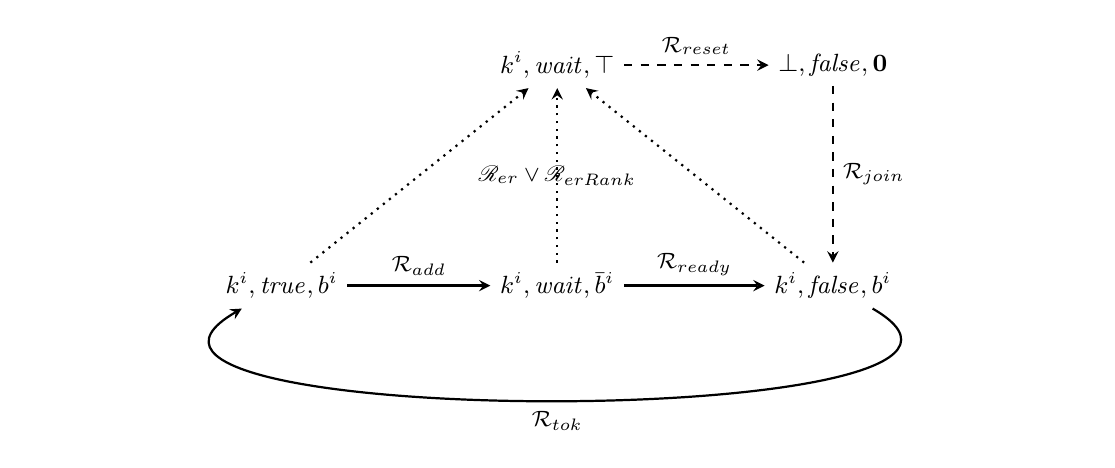
\begin{tikzpicture}[
  every node/.style={font=\small},
  state/.style={draw=none},
  arr/.style={->, >=stealth, thick},
  redarr/.style={arr, color=red!70!black},
  pinkarr/.style={arr,dotted},
  bluearr/.style={arr,dashed},
]

\node[state] (A) at (0,0)   {$\rk^i, \mathit{true}, b^i$};
\node[state] (B) at (3.5,0) {$\rk^i, \mathit{wait}, \bar{b}^i$};
\node[state] (C) at (7,0)   {$\rk^i, \mathit{false}, b^i$};
\node[state] (E) at (3.5,2.8) {$\rk^i, \mathit{wait}, \top$};
\node[state] (R) at (7,2.8) {$\bot, \mathit{false}, \mathbf{0}$};



\draw[arr] (A) -- node[above]{\footnotesize$\mathcal{R}_{add}$} (B);
\draw[arr] (B) -- node[above]{\footnotesize$\mathcal{R}_{ready}$} (C);
\draw[arr] (C) to[out=-30, in=-150] 
  node[below]{\footnotesize$\mathcal{R}_{tok}$} (A);

\draw[pinkarr] (A) -- 
   (E);
\draw[pinkarr] (B) -- node{\footnotesize $\Rer \vee \RerRank$}(E);
\draw[pinkarr] (C) -- (E);


\draw[bluearr] (E) -- node[above]{\footnotesize$\mathcal{R}_{reset}$} (R);

\draw[bluearr] (R) to 
  node[right]{\footnotesize$\mathcal{R}_{join}$} 
  (C);

\end{tikzpicture}
\caption{Transition graph of the rules of $\mathtt{TokBinV}$, where 
$\rk^i \in \{0,1,2\}$ and $b^i \in \{\mathbf{0},\mathbf{1}\}$; 
$\bar{b}^i$ denotes the bit obtained by flipping $b^i$, 
i.e., $\bar{b}^i = (b^i + 1) \bmod 2$. }
\label{fig:transition-rules}
\end{figure}

\paragraph{狀態轉移圖}
轉移圖以三元組 \((\rk_v,t_v,b_v)\) 表示所有可能狀態轉移：
\begin{itemize}
    \item 正常循環：\((\rk^i,\mathit{true},b^i)\xrightarrow{\Radd}(\rk^i,\mathit{wait},\bar{b}^i)\xrightarrow{\Rready}(\rk^i,\mathit{false},b^i)\xrightarrow{\Rtok}(\rk^i,\mathit{true},b^i)\)。
    \item 錯誤路徑：任何狀態經 \(\Rer\vee\RerRank\) 到 \((\rk^i,\mathit{wait},\top)\)，再經 \(\Rreset\) 到 \((\bot,\mathit{false},\bz)\)，最後經 \(\Rjoin\) 回到正常。
\end{itemize}
其中 \(\bar{b}^i=(b^i+1)\bmod 2\)。

\paragraph{權杖傳遞示意（圖 5）}
\begin{itemize}
    \item \textbf{(a)} \(v\) 持有並提供權杖；\(u\) 經 \(\Rtok\) 取得，\(v\) 經 \(\Radd\) 遞增位元。
    \item \textbf{(b)} \(v\) 經 \(\Rready\) 表示準備好；\(u\) 持有權杖，經 \(\Radd\) 釋放並遞增；同時 \(w\) 經 \(\Rtok\) 取得。
    \item \textbf{(c)} \(u\) 執行 \(\Rready\)；\(w\) 持有並執行 \(\Radd\)；\(x\) 經 \(\Rtok\) 取得。
    \item \textbf{(d)} \(x\) 持有並執行 \(\Radd\)；但 \(y\) 無法取得，因 \(b_x=\bz\)。
    \item \textbf{(e)} \(x\) 執行 \(\Rready\)。
\end{itemize}

\section{Correctness（正確性）}

\subsection{Space Complexity（空間複雜度）}

\subsection{Definitions and Notations（定義與符號）}

\subsection{Overview of Correctness（正確性概述）}

\subsection{Root Stabilization ($\Gamma_r$)（根節點穩定化）}
\label{sec:root}

\subsection{Obvious Errors ($\Gamma_{\bar{e}}$)（明顯錯誤）}
\label{subsec:obvious}

\subsection{Legal Configurations: Definitions and Properties（合法配置：定義與性質）}
\label{sec:legal}

\subsection{Closure of Legal Configurations（合法配置的封閉性）}
\label{sec:closure}

\subsection{Initial Tokens Lifetime ($\Gamma_{\bar{it}}$)（初始令牌生命期）}
\label{subsec:tokenlifetime}

\subsection{Legal Rank（合法秩）}
\label{subsec:legalrank}

\subsection{Token Dissemination（令牌散播）}
\label{sec:tokDis}

\subsection{Residual Error Removal ($\Gamma_{cl}$)（殘餘錯誤移除）}
\label{subsec:residual}

\subsubsection{Cleaner Wave（清理波）}
\label{subsub:clean}

\subsubsection{Legal Rank Wave（合法秩波）}
\label{subsub:goodrank}

\subsubsection{Legal Path Wave（合法路徑波）}
\label{subsub:legalpath}

\subsubsection{Proof of Residual Error Removal（殘餘錯誤移除之證明）}
\label{subsub:proofclean}

\subsection{Convergence to Legal Configurations ($\Gamma^*$)（收斂至合法配置）}
\label{subsec:convergencelegal}

\section{Concluding Remarks（結論）}

% \bibliographystyle{plain}
% \bibliography{biblio}

\end{document}